\documentclass[parskip=half,DIV=12,bookmarkpackage=false]{scrartcl}

\title{Lab assignment 2}
\subtitle{ATM S 544}
\author{Dominik Stiller}
\date{\today}

\usepackage[english]{babel}
\usepackage[utf8]{inputenc}
\usepackage{siunitx,amsmath,physics}
\usepackage{caption,subcaption,graphicx,csquotes,xcolor}
\usepackage{booktabs}
\usepackage{placeins}
\usepackage[
	backend=biber,
	bibwarn=true,
	bibencoding=utf8,
	sortlocale=en_US,
	url=false,
	style=apa,
	isbn=false
]{biblatex}

\definecolor{uw-purple}{RGB}{51, 0, 111}

\usepackage{hyperref}
\hypersetup{
	% hidelinks,
	colorlinks=true,
	linkcolor=black,
	citecolor=black,
	urlcolor=uw-purple
}

\usepackage{doi}
\usepackage{nomencl}
\makenomenclature
\usepackage[noabbrev,capitalise]{cleveref}
\usepackage[acronym,nonumberlist,nopostdot,nogroupskip]{glossaries}
\usepackage[
	outputdir=build,
]{minted}
\setminted{
	linenos,
	tabsize=4,
	fontsize=\small,
}
\newmintinline{python}{}

\usepackage{lmodern}
\usepackage[T1]{fontenc}
\usepackage{inconsolata}
\usepackage{tikz}

\newcommand{\result}[1]{\colorbox{uw-purple}{\textcolor{white}{#1}}}

\setlength{\nomlabelwidth}{1.5cm}
\setlength{\nomitemsep}{-\parsep}
\newcommand{\nomunit}[1]{%
\renewcommand{\nomentryend}{\hspace*{\fill}\si{#1}}}

\sisetup{per-mode=symbol}
\AtBeginDocument{\RenewCommandCopy\qty\SI}

\DeclareGraphicsRule{.ai}{pdf}{.ai}{}

\addbibresource{bibliography.bib}



\begin{document}

\maketitle




\section{Gaussian distribution}
\label{sec:gaus}


\begin{figure}[ht]
    \centering
    
    \begin{subfigure}[c]{0.49\textwidth}
        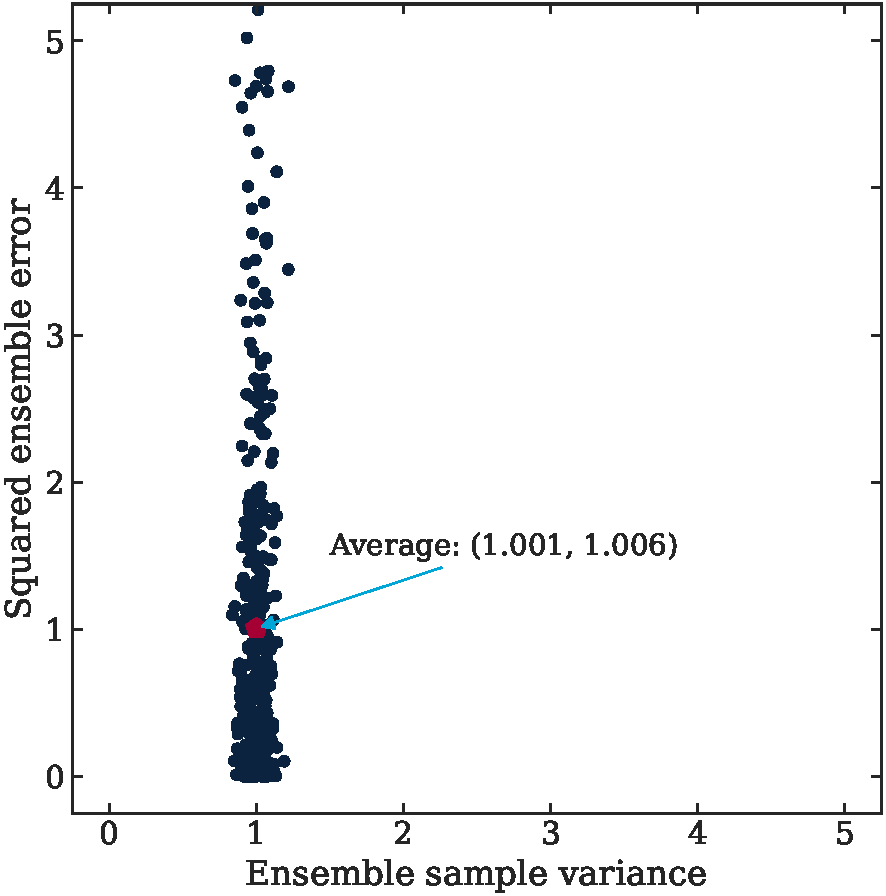
\includegraphics[width=\textwidth]{figures/var_vs_err_1.00.pdf}
        \subcaption{$\sigma_v^2 = 1$}
        \label{fig:var-1}
    \end{subfigure}
    \hfill
    \begin{subfigure}[c]{0.49\textwidth}
        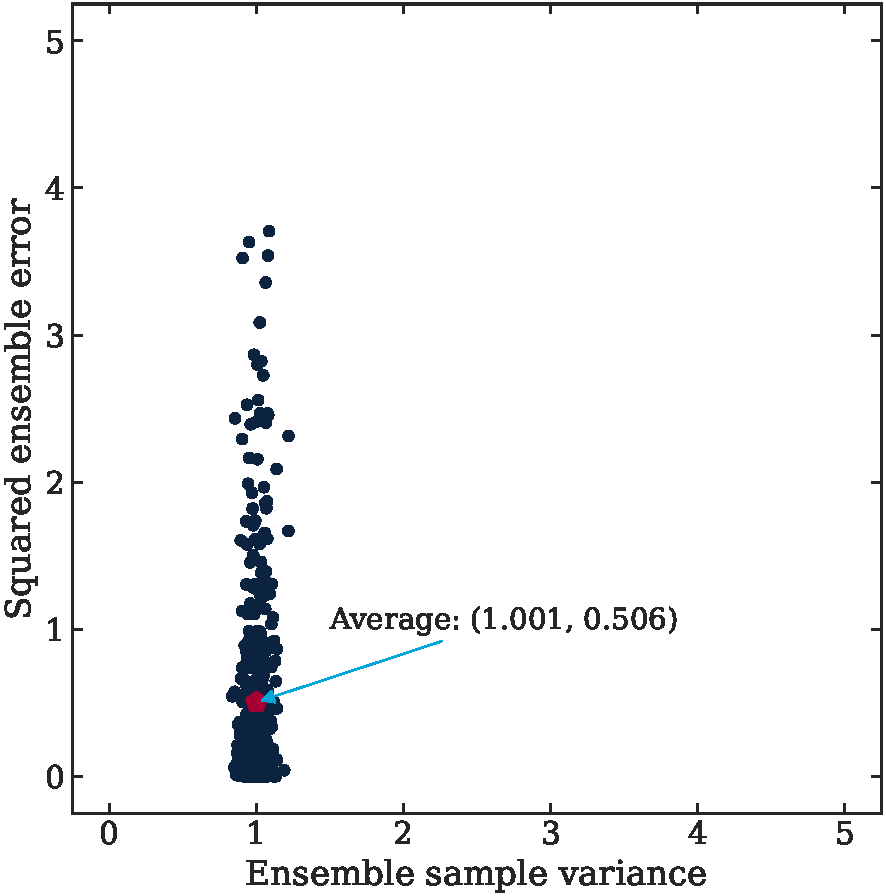
\includegraphics[width=\textwidth]{figures/var_vs_err_0.50.pdf}
        \subcaption{$\sigma_v^2 = 0.5$}
        \label{fig:var-05}
    \end{subfigure}
 
    \caption{Variance vs. squared error for $N_e = 500$ and $N_c = 500$. The ensemble is drawn from $\mathcal{N}(0, 1)$, the verification from $\mathcal{N}(0, \sigma_v^2)$.}
 \end{figure}

%  The raison d'être for ensembles is the estimation of uncertainty and variability. The ensemble spread is used as proxy for the confidence in the point estimate given by the mean, or rather, it allows to express the estimate probabilistically.

 \cref{fig:var-1} shows the ensemble spread compared to the error w.r.t.\ the verification. Since we use a large ensemble of $N_e = 500$ members, the spread is rather small and converged to the true variance of $1$. Since the ensemble members and verification are drawn from the same distribution (i.e., the forecast model is a good approximation of reality), the average ensemble sample variance coincides with the average squared error over all $N_c = 500$ cases.

 \cref{fig:var-05} shows the case where the ensemble spread overestimates the true variability (i.e., the forecast model does not approximate real variability well, even though the true and estimated mean still coincide). The estimate still predicts a sample variance of $1$, but the actual average squared error is just $0.5$.





 \section{PanguWeather}

 \begin{figure}[ht]
    \centering
    
    \begin{subfigure}[c]{0.49\textwidth}
        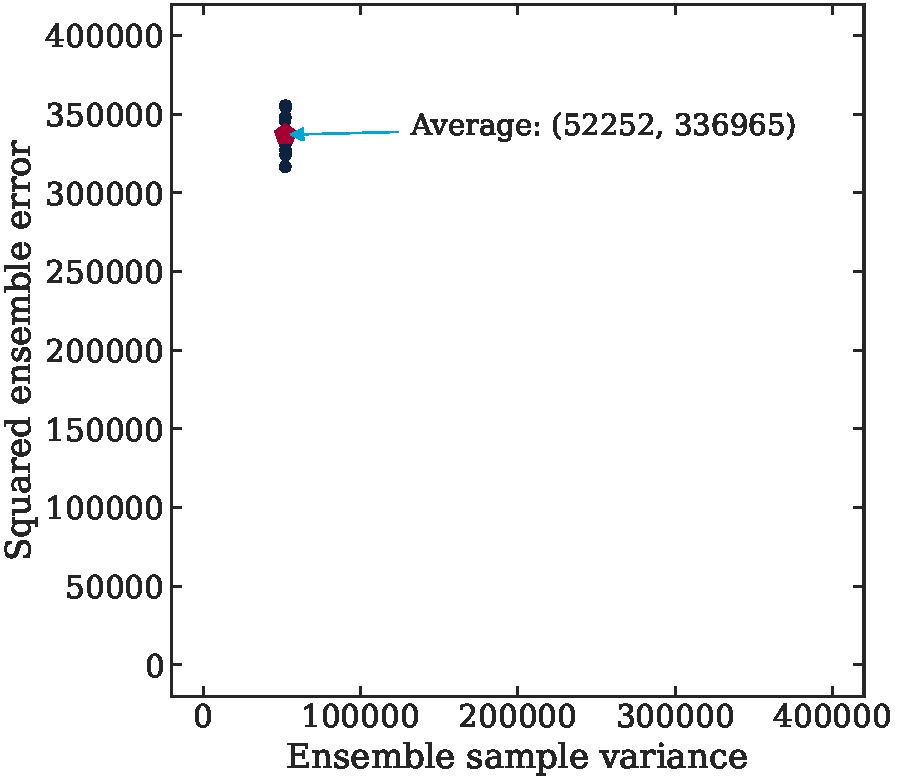
\includegraphics[width=\textwidth]{figures/var_vs_err_pangu_ens.pdf}
        \subcaption{Ensemble member \# 1 verification}
        \label{fig:pangu-ens}
    \end{subfigure}
    \hfill
    \begin{subfigure}[c]{0.49\textwidth}
        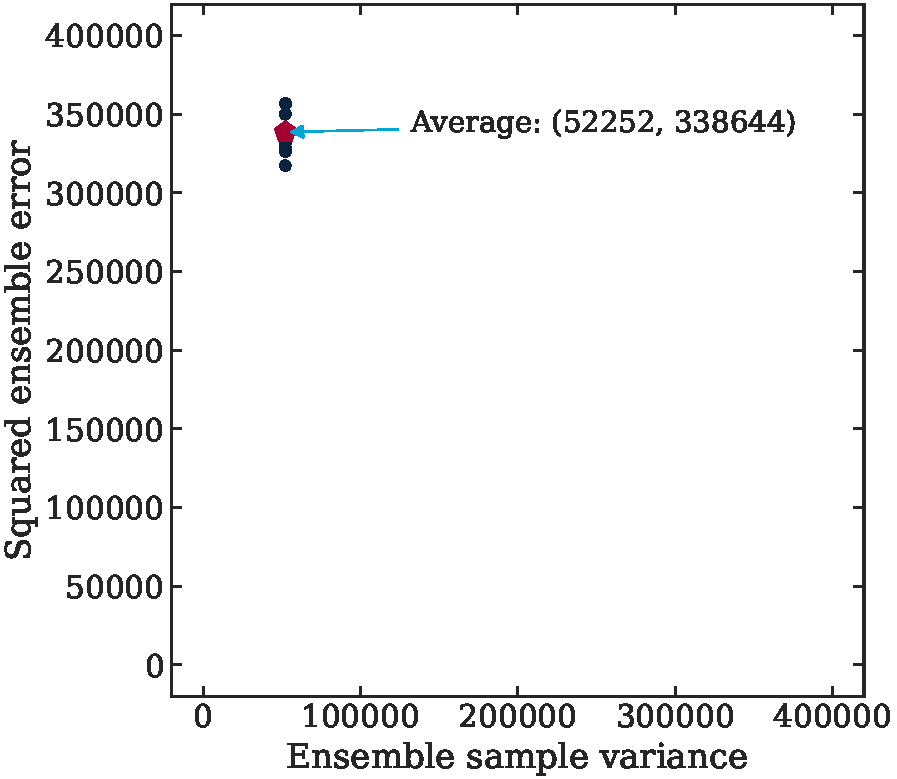
\includegraphics[width=\textwidth]{figures/var_vs_err_pangu_era5.pdf}
        \subcaption{ERA5 verification}
        \label{fig:pangu-era}
    \end{subfigure}
    
    \caption{Variance vs. squared error in Z500 geopotential for $N_e = 4$ and $N_c = 10$.}
    \label{fig:pangu}
 \end{figure}

 For the PanguWeather forecast, the first ensemble member has an unperturbed initial condition, the other four have a noise amplitude of 0.05. We verify both against the first ensemble member (same distribution, similar to case 1) and against ERA5 (different distribution, similar to case 2).

 \Cref{fig:pangu} shows the ensemble spread compared to the error w.r.t.\ the verification. Interestingly, the squared ensemble error in both cases is virtually identical. This indicates that PanguWeather, which has been trained on ERA5, indeed has learned the forecast relationship over 24 h. However, the ensemble sample variance is off by a factor 7. Both cases therefore resemble case 2 from before, where the model does not capture the true variability. Possibly, this is because of a small ensemble size of $N_e = 4$. Still, the discrepancy is very large and may have another explanation.
 



\end{document}
